\chapter{工程实际问题}
在本章中对三角板减振刚度阻尼器施加受力,
\section{TADAS阻尼器}
三角板减振刚度阻尼器(TADAS阻尼器)是一种广泛应用于结构工程中用于减震和控制结构的主动控制装置,其具有减少结构在地震、风荷载或其他动力荷载作用下的振动幅值和响应,相较于传统的被动阻尼器,TADAS阻尼器具有更高的阻尼效率,具有可调性和自适应性。
为了更好将本文提出的方法与工程实际相结合,利用[]中对TADAS阻尼器进行建模,分析基于Hellinger-Reissner原理的变分一致型伽辽金无网格法的计算效果。
\par
图(\ref{TADAS1})为一层一湾框架的大比例模型,在道路、住房和城市发展研究中心建造。框架高3米,跨度4米,框架柱采用标准的双IPE180型钢材,梁的工字截面由三块4000*200*12mm的钢板连续焊接而成。支撑体系统一采用双100*100*20mm角度,柱基座使用销连接。
图(\ref{TADAS2})表示为框架模型中的TADAS阻尼器示意图,使用V形支撑系统集成到机构中。
\begin{figure}[H]
    \centering
    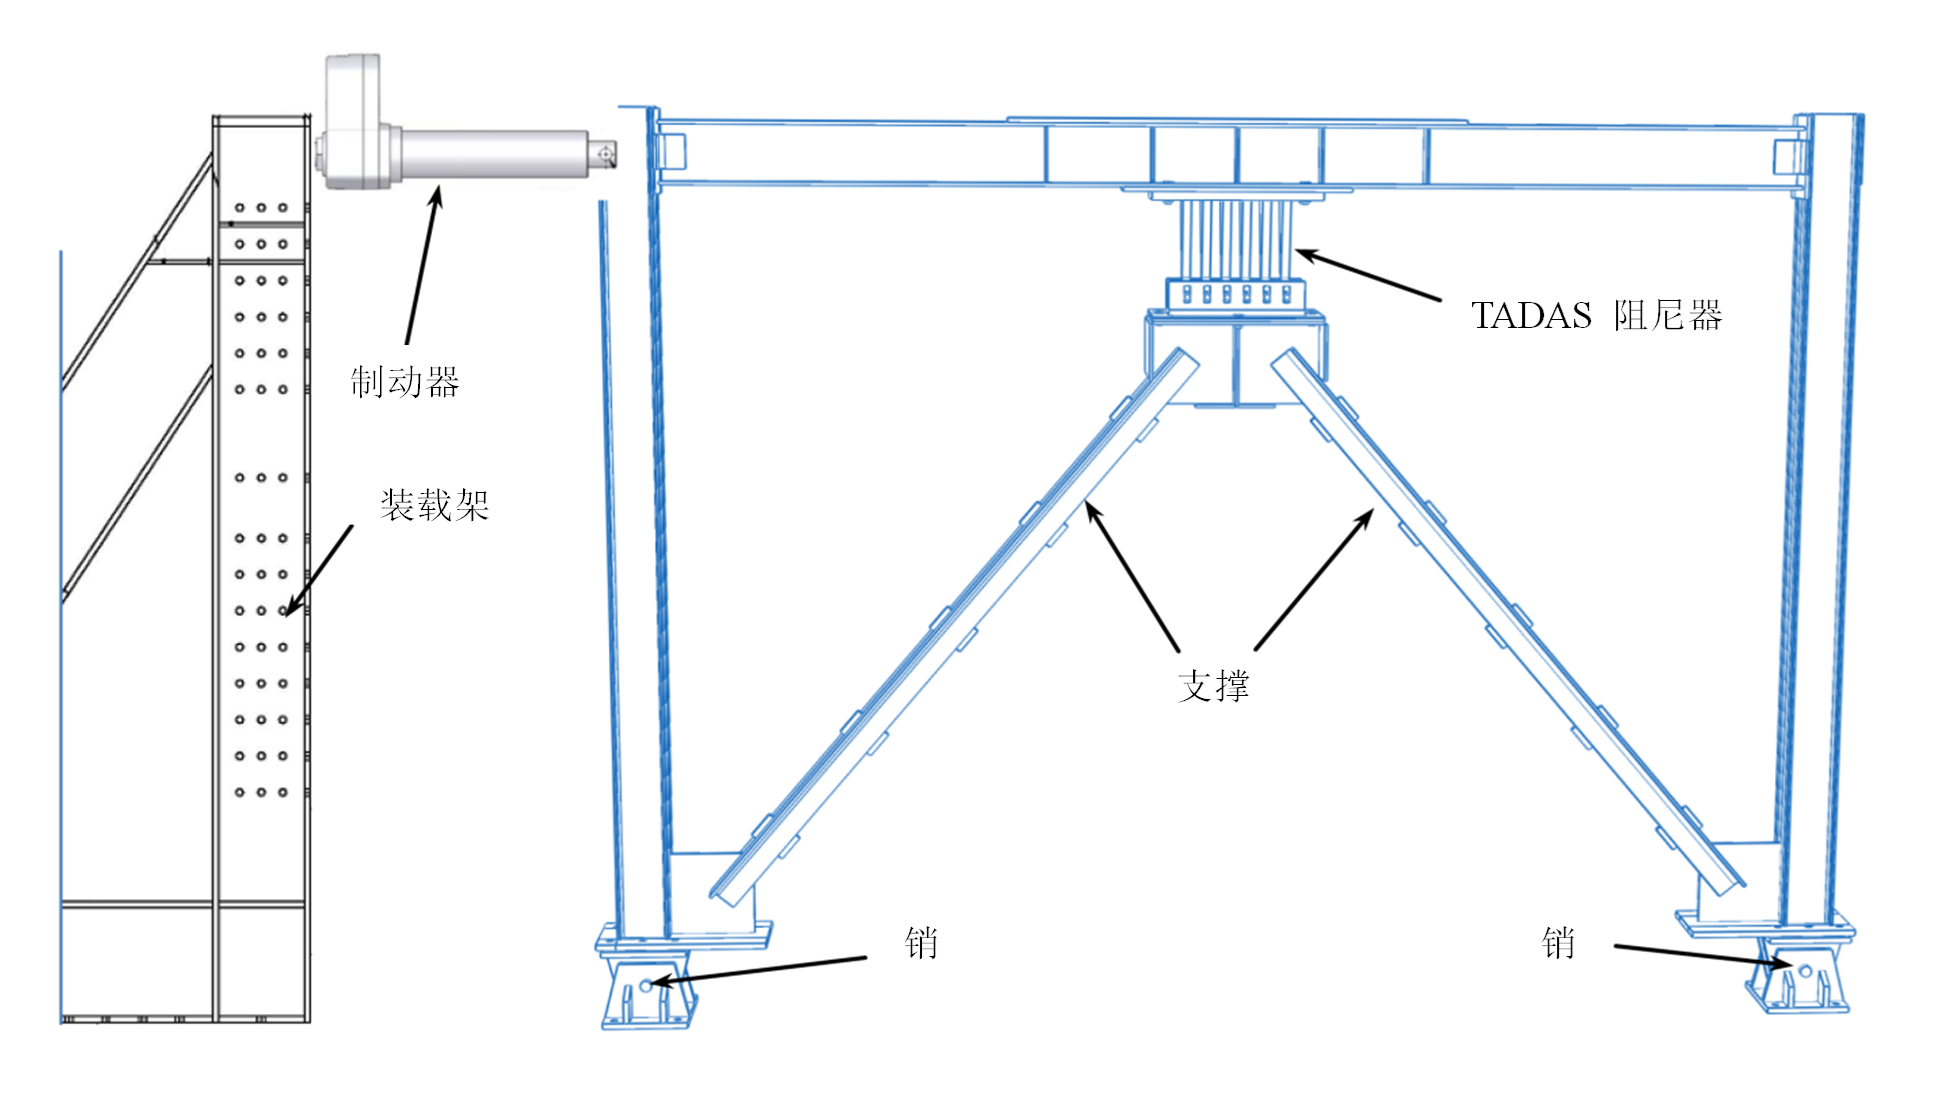
\includegraphics[scale=0.4]{figure/TADAS/1.png}
    \caption{实验装置示意图}\label{TADAS1}
\end{figure}
\begin{figure}[H]
    \centering
    \begin{subcaptiongroup}
            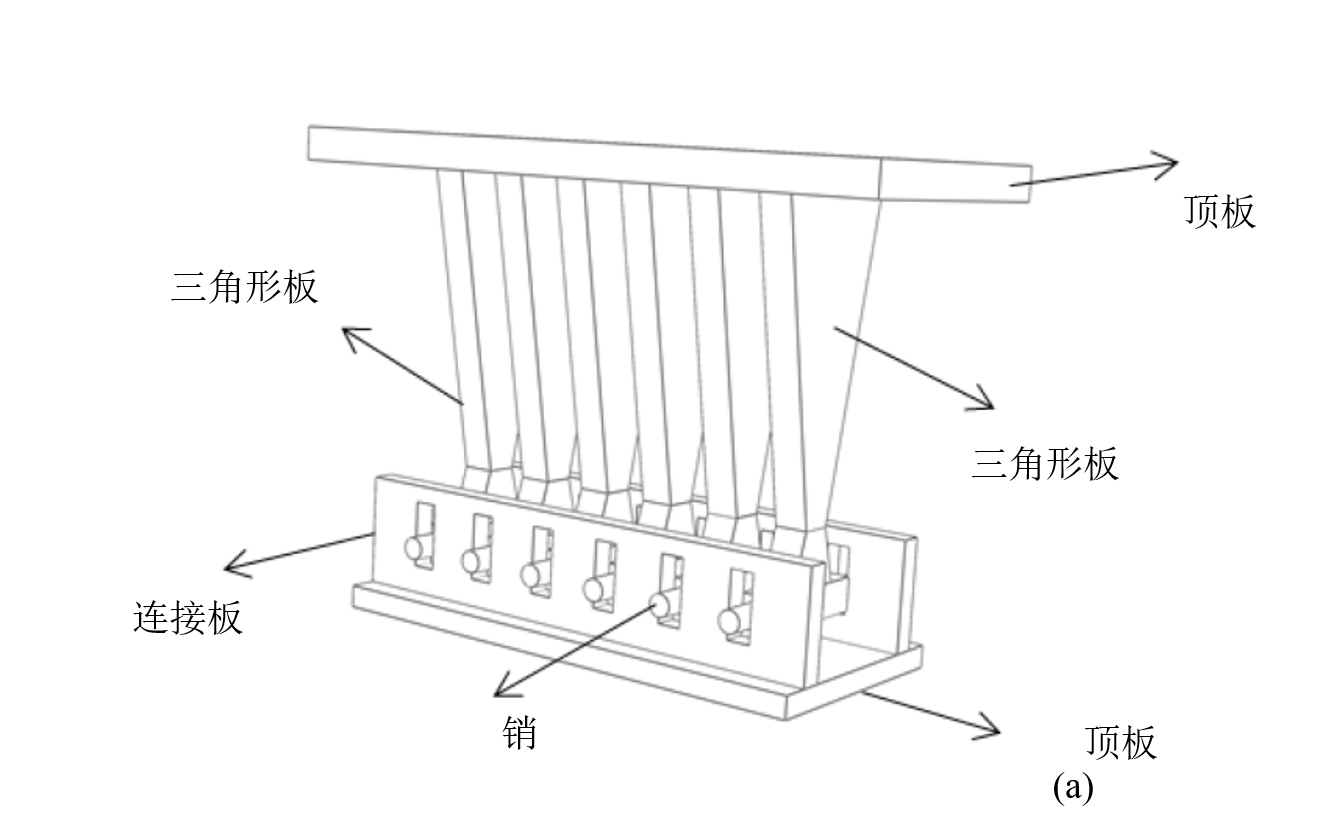
\includegraphics[width=0.69\textwidth]{figure/TADAS/2.png}
            \phantomcaption\label{TADAS2}
            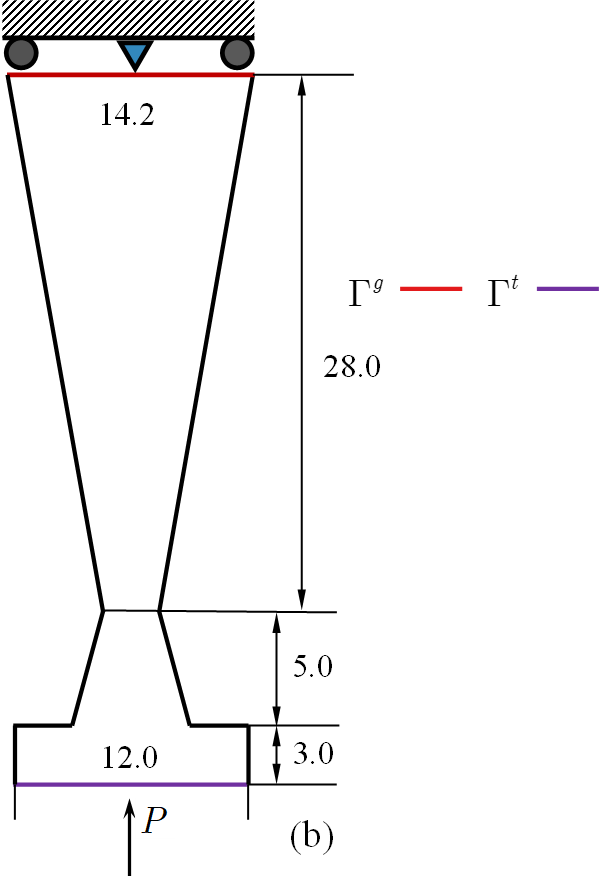
\includegraphics[width=0.29\textwidth]{figure/TADAS/3.png}
            \phantomcaption\label{TADAS3}
            \end{subcaptiongroup}
        \caption{TADAS阻尼器示意图:\subref{TADAS2} 钢板焊接TADAS装置详图;\subref{TADAS3} 三角形钢板横截面图}
    \label{TADAS2}
\end{figure}


